\documentclass{exam}
\usepackage[utf8]{inputenc}
\usepackage{lmodern}
\usepackage{microtype}

% \usepackage[parfill]{parskip}
\usepackage[dvipsnames]{xcolor}
\usepackage{amsmath}
\usepackage{amsfonts}
\usepackage{amsthm}
\usepackage{siunitx}
\DeclareSIUnit\year{yr}
\DeclareSIUnit\foot{ft}
\DeclareSIUnit\litre{\liter}

\usepackage{skull}

\usepackage{pgfplots}
\usepgfplotslibrary{polar}
\pgfplotsset{compat=1.11}
\usepgfplotslibrary{statistics}
\usepackage{graphicx}
\usepackage{sidecap}
\sidecaptionvpos{figure}{c}
\usepackage{float}
\usepackage{gensymb}
\usepackage{tkz-euclide}
\usetkzobj{all}
\usepackage{commath}
\usepackage{hyperref}
\usepackage{enumitem}
\usepackage{wasysym}
\usepackage{multicol}
\usepackage{mathtools}
\usepackage{tcolorbox}
\usepackage{tabularx}
\usepackage[version=4]{mhchem}
\usepackage{changepage}
\usepackage{listings}
\lstset{basicstyle=\ttfamily\linespread{0.8}\small}

\renewcommand*{\thefootnote}{\fnsymbol{footnote}}

\newtheorem*{thm}{Theorem}
\newtheorem*{iden}{Identity}
\newtheorem*{lemma}{Lemma}
\newtheorem{obs}{Observation}
\theoremstyle{definition}
\newtheorem*{defn}{Definition}
\newtheorem*{ex}{Example}
\newtheorem{con}{Construction}
\newtheorem*{alg}{Algorithm}

\newtheoremstyle{break}
  {\topsep}{\topsep}%
  {\itshape}{}%
  {\bfseries}{}%
  {\newline}{}%
\theoremstyle{break}
\newtheorem*{bthm}{Theorem}

% russian integral
\usepackage{scalerel}
\DeclareMathOperator*{\rint}{\scalerel*{\rotatebox{17}{$\!\int\!$}}{\int}}

% \DeclareMathOperator*{\rint}{\int}

\pgfplotsset{vasymptote/.style={
    before end axis/.append code={
        \draw[densely dashed] ({rel axis cs:0,0} -| {axis cs:#1,0})
        -- ({rel axis cs:0,1} -| {axis cs:#1,0});
    }
}}

% \pointsinrightmargin
\boxedpoints
\pointname{}

\newcommand{\questioA}{\question[\texttt{\textbf{\color{Cerulean} A}}]}
\newcommand{\questioM}{\question[\texttt{\textbf{\color{PineGreen} M}}]}
\newcommand{\questioE}{\question[\texttt{\textbf{\color{WildStrawberry} E}}]}
\newcommand{\questioS}{\question[\texttt{\textbf{\color{Goldenrod} S}}]}
\newcommand{\questioO}{\question[\texttt{\textbf{\color{BurntOrange} O}}]}

\newcommand{\parA}{\part[\texttt{\textbf{\color{Cerulean} A}}]}
\newcommand{\parM}{\part[\texttt{\textbf{\color{PineGreen} M}}]}
\newcommand{\parE}{\part[\texttt{\textbf{\color{WildStrawberry} E}}]}
\newcommand{\parS}{\part[\texttt{\textbf{\color{Goldenrod} S}}]}
\newcommand{\parO}{\part[\texttt{\textbf{\color{BurntOrange} O}}]}

\newcommand{\subparA}{\subpart[\texttt{\textbf{\color{Cerulean} A}}]}
\newcommand{\subparM}{\subpart[\texttt{\textbf{\color{PineGreen} M}}]}
\newcommand{\subparE}{\subpart[\texttt{\textbf{\color{WildStrawberry} E}}]}
\newcommand{\subparS}{\subpart[\texttt{\textbf{\color{Goldenrod} S}}]}
\newcommand{\subparO}{\subpart[\texttt{\textbf{\color{BurntOrange} O}}]}

\newcommand{\mainHeader}[2]{\section*{NCEA Level 2 Mathematics\\#1. #2}}
\newcommand{\mainHeaderHw}[2]{\section*{NCEA Level 2 Mathematics (Homework)\\#1. #2}}
\newcommand{\seealso}[1]{\begin{center}\emph{See also #1.}\end{center}}
\newcommand{\drills}[1]{\begin{center}\emph{Drill problems: #1.}\end{center}}
\newcommand{\basedon}[1]{\begin{center}\emph{Notes largely based on #1.}\end{center}}

\begin{document}

\mainHeaderDiffHw{7}{Higher Derivatives and the Geometry of a Function}
\subsection*{Reading}
\begin{center}
  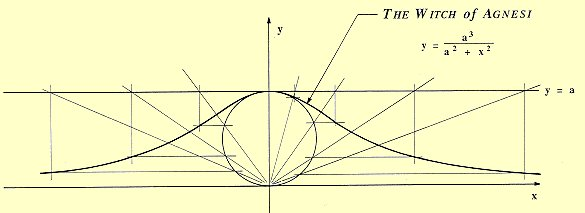
\includegraphics[width=0.7\textwidth]{agnesi-curve}

  \vspace{2mm}
  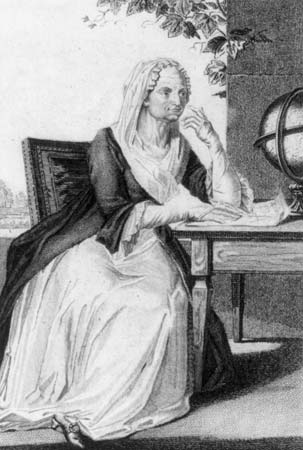
\includegraphics[width=0.3\textwidth]{agnesi}
\end{center}

Maria Gaetana Agnesi (1718 - 1799) was an Italian mathematician and philosopher, considered to be the first woman in the Western world to have achieved a reputation in mathematics.

Agnesi was the eldest child of a wealthy silk merchant who provided her with the best tutors available. She was an extremely precocious child who mastered Latin, Greek, Hebrew, and several modern languages at an early age, and her father liked to host gatherings where she could display her knowledge. Propositiones philosophicae (“Propositions of Philosophy”), a series of essays on natural philosophy and history based on her discussions before such gatherings, was published in 1738.

Agnesi’s best-known work, \textit{Instituzioni analitiche ad uso della gioventù italiana} (1748; “Analytical Institutions for the Use of Italian Youth”), in two huge volumes, provided a remarkably comprehensive and systematic treatment of algebra and analysis, including such relatively new developments as integral and differential calculus. In this text is found a discussion of the Agnesi curve, a cubic curve known in Italian as versiera, which was confused with versicra (“witch”) and translated into English as the “Witch of Agnesi.” The French Academy of Sciences, in its review of the Instituzioni, stated that: “We regard it as the most complete and best made treatise.” Pope Benedict XIV was similarly impressed and appointed Agnesi professor of mathematics at the University of Bologna in 1750.

However, Agnesi had turned increasingly to religion and never journeyed to Bologna. After the death of her father in 1752, she devoted herself almost exclusively to charitable work and religious studies. She established various hospices and died in one of the poorhouses that she had once directed.

\textit{From \url{https://www.britannica.com/biography/Maria-Gaetana-Agnesi}.}

\subsection*{Questions}
\begin{questions}
  \question Explain the geometric meaning of the second derivative.
  \question Find the second derivative of the following functions.
    \begin{parts}
      \part $ f(x) = x^5 - 5x + 3 $
      \part $ f(x) = \frac{x^2}{x - 1} $
      \part $ f(x) = \sqrt{x} - \sqrt[4]{x} $
    \end{parts}
  \question Sketch a function satisfying the given criteria.
    \begin{parts}
      \part (hint: your result should be an odd function)
        \begin{subparts}
           \subpart $ f'(1) = f'(-1) = 0 $,
           \subpart $ f'(x) < 0 $ if $ \abs{x} < 1 $,
           \subpart $ f'(x) > 0 $ if $ 1 < \abs{x} < 2 $,
           \subpart $ f'(x) = -1 $ if $ \abs{x} > 2 $.
        \end{subparts}
      \part
        \begin{subparts}
          \subpart $ f'(x) < 0 $,
          \subpart $ f''(x) < 0 $.
        \end{subparts}
    \end{parts}
\end{questions}
\end{document}
